\begin{abstract}
	Les algorithmes génétiques appartiennent à la famille des algorithmes évolutionnistes. Ils permettent d'obtenir une solution approchée ou exacte à un problème d'optimisation. Au nombre de ces algorithmes génétiques figurent une catégorie connue sous le nom d'algorithmes génétiques parallèles. De plus, en combinant ces différents algorithmes génétiques parallèles \cite{cant2}, l'on obtient alors des algorithmes génétiques parallèles et hiérarchiques encore plus efficaces. 
\end{abstract}

\section*{Introduction}
	\addcontentsline{toc}{section}{Introduction}
	 Dans ce chapitre, nous présentons dans un premier temps nos outils de test, puis le modèle utilisée dans notre étude afin de représenter les instances de PSP et ensuite les aspects généraux ou communs à nos deux approches heuristiques basées sur les algorithmes génétiques. Dans un second temps, nous décrivons ces deux méthodes de recherche en nous appuyant sur les algorithmes implémentés.
	
	\section{Outils de test} 
		\subsection{Matériel}
		Pour l'implémentation de nos tests, nous avons travaillé sur un ordinateur présentant les caractéristiques suivantes :\\
		\begin{itemize}
			\item[•] Système d'exploitation: Linux Ubuntu 16.04 LTS; \\
			\item[•] Processeur: Intel®  Core \up{\textsc{TM}} i7 CPU L 640 @ 2.13GHz x 4; \\
			\item[•] Mémoire: 3,7 Gio;\\
			\item[•] Type du système d'exploitation: 64 bits.\\
		\end{itemize}
		
		\subsection{Langage de programmation}
		Le langage de programmation utilisée afin d'implémenter nos deux approches est le langage \emph{Python} dans sa version Python 3.5. \emph{Python} est un langage de programmation interprété et orienté objet. Il est placé sous une licence libre et fonctionne sur la plupart des plates-formes informatiques \cite{wikipedia_python}.
	
	\section{Modèle et formulation utilisés}
	Dans le but de modéliser et de formuler les instances de PSP, nous nous sommes servis de la première formulation en programmation en nombres entiers (MIP1). Nous rappelons ici ce modèle. 
	
	\begin{eqnarray}
		min \sum_{i,j,t} q^{i,j}ch_{t}^{i,j} + \sum_{i,t} h^{i} s_{t}^{i} \\
		s_{0}^{i} = 0, \forall i \\
		x_{t}^{i} + s_{t-1}^{i} = d_{t}^{i} + s_{t}^{i}, \forall i,t \\
		x_{t}^{i} \leq y_{t}^{i}, \forall i,t \\
		\sum_{i} y_{t}^{i} = 1 , \forall t \\
		\chi_{t}^{i,j} = y_{t-1}^{i} + y_{t}^{j} - 1, \forall i,j,t \\
		x,y,\chi \in \{0,1\}, s \in N, i \in \{0..NI\}, t \in \{1..NT\}
	\end{eqnarray}
		
		avec les variables de décisions suivantes: \\
		\begin{itemize}
			\item[-] $x_{t}^{i}$ : variable binaire de production qui vaut 1 si l’article $i$ est produit à la période $t$ et 0 sinon ;
			\item[-] $y_{t}^{i}$ : variable binaire de setup qui vaut 1 si la machine est préparée pour la production de l’article $i$ et 0 sinon ;
			\item[-] $s_{t}^{i}$ : variable entière de stockage qui contient le nombre d’articles $i$ stockés à la période $t$ ; 
			\item[-] $\chi_{t}^{i,j}$ : variable binaire de transition qui vaut 1 si à la période $t$, on est passé de la production de l’article $i$ à l’article $j$ et 0 sinon.
		\end{itemize}
	
	\section{Aspects généraux aux deux méthodes de recherche proposées}
	\subsection{Représentation génétique}
	Différentes représentations peuvent être utilisées avec les techniques évolutionnaires telles que les algorithmes génétiques. La représentation la plus simple pour les algorithmes génétiques est celle utilisée par John Holland: une chaîne de bits. Une chaîne de bits est connue comme un chromosome, et chaque bit est un gène. En début d'étude, nous avons donc commencé par représenter un chromosome en chaîne de bits. \\
	\textsl{\textbf{Exemple}}:\\
	\hspace*{.5cm} En suivant l'exemple d'une instance de PSP en page \pageref{sec:problem_description}, nous pouvons représenter un chromosome conformément à la figure \ref{fig:init_gene_repr}.
	
	\begin{figure}[h]
		\begin{center}
			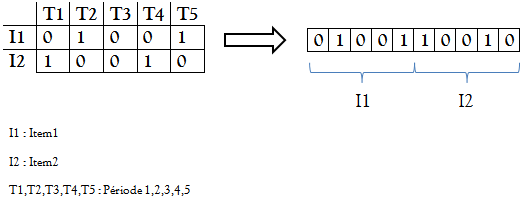
\includegraphics[scale=.5]{images/init_gene_repr.png}
			\caption{Représentation génétique initiale}
			\label{fig:init_gene_repr}
		\end{center}
	\end{figure}
	
	Autrement dit:
	\begin{center}
		$ch_{T} = \{(x_{1,1}),..., (x_{1,t+1}),..., ( x_{1,T}), (x_{i+1,1}),...,(x_{i+1, t+1}),..., (x_{i+1,T}),..., (x_{I,T})\}$ \\
	\end{center}
	\hspace*{.5cm} où $x_{it}$ est la variable booléenne qui indique la production ou non d'un article \emph{i} en période \emph{t}.  \\
	\\
	\hspace*{.5cm} Dans cette représentation, un chromosome est une chaîne de bits (0 et 1) qui indique la production ou non d'un article \emph{i} et de longueur \emph{nItems * nTimes} (où \emph{nItems} est le nombre d'articles et \emph{nTimes} est le nombre de périodes). Ainsi, l'article 1 est produit dans les périodes 2 et 5; et l'article 2 est produit dans les périodes 1 et 4. Le chromosome représenté ci-dessus est ainsi un plan de production qui satisfait aux contraintes du système de production spécifiques à cette instance du problème. Toutefois, au cours de notre étude, une seconde représentation nous est apparue plus cohérente et facilement manipulable. Cette représentation génétique est présentée à la figure \ref{fig:adopt_gene_repr} et étudiée par Mirshekarian et al. \cite{suer}.
	
	\begin{figure}[!h]
		\begin{center}
			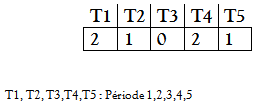
\includegraphics[scale=.5]{images/adopt_gene_repr.png}
			\caption{Représentation génétique adoptée}
			\label{fig:adopt_gene_repr}
		\end{center}
	\end{figure}
	
	Dans cette représentation, un chromosome est une suite d'entiers correspondant aux articles produits et de longueur \emph{nTimes}. La longueur réduite de ce chromosome réduit dans le même temps la durée du parcours du chromosome lors des implémentations.
	\subsection{Initialisation}
	Le processus d'initialisation consiste à construire la population initiale; c'est à dire celle à partir de laquelle se feront les opérations de sélection, croisement ou encore mutation afin de la faire évoluer sur des générations. L'initialisation au niveau des algorithmes génétiques se fait de manière aléatoire dans l'optique de trouver des individus suffisamment différents capables de constituer une population diverse dans le but de largement couvrir l'espace de recherche. \\
	\hspace*{.5cm} Une autre approche consiste à créer les individus devant composer la population initiale en se servant de stratégies de recherche déterministes et informés munis de fonctions d'évaluation suffisamment précises menant à des bonnes solutions. Notre approche a été donc d'utiliser une stratégie de recherche en l’occurrence le "Hill Climbing" dotée d'une fonction d'évaluation afin de déterminer lequel des fils à considérer.\\
	\hspace*{.5cm} \textbf{\textsl{Principe:}}\\
	Le principe d'initialisation de la population est le suivant : remplir un chromosome en commençant par le dernier gène et en finissant par le premier. Cela permet de s'assurer de la faisabilité des solutions que nous trouvons au bout du processus. Ainsi, pour chaque gène visité, nous disposons de la liste des allèles qui peuvent prétendre occuper ce dernier, nous pouvons alors choisir l'allèle qui minimise le "fitness" du chromosome en train d'être constitué.\\
	\hspace*{.5cm} \textbf{\textsl{Algorithme:}}\\	
	L'algorithme \ref{alg:generation_pop_init} détaille le processus de génération de la population initiale: \\
	
	\begin{algorithm}[H]
		\caption{Processus de génération de la population initiale}
		\label{alg:generation_pop_init}
 		\KwData{instance de PSP à traiter, taille de la population}
 		\BlankLine
 		\KwResult{Population initiale constituée}
		\BlankLine 		
		$queue \gets []$
		\BlankLine
		$noeud \gets nouveauNoeud()$ \\
		\BlankLine
 		\While{taille(populationInitiale) est inférieure à taillePopulation}{
 			\BlankLine
 			\eIf{noeud.chromosome est prêt}{
 				\BlankLine
 			 	populationInitiale.ajouter(noeud.chromosome)
 			 	\BlankLine
 			 }
 			 {
 			 	\BlankLine
 			 	$noeudFils \gets noeud.getSuccessors()$ \\
 			 	\BlankLine
 			 	noeudFils.trier(decroissant) \\
 			 	\BlankLine
 			 	queue.ajouter(noeudFils)
 			 	\BlankLine
 			 	\If {queue est vide}
 			 	{
 			 		\BlankLine
 			 		\Return populationInitiale
 			 		\BlankLine
 			 	}
 			 	\BlankLine
 			 	$noeud \gets  queue.dernier()$
 			 }	
	}
	\Return populationInitiale
	\end{algorithm}	
	L'algorithme \ref{alg:generation_successeurs} décrit la génération des successeurs d'un noeud donné.
	\begin{algorithm}
		\caption{Processus de génération des successeurs d'un noeud}
		\label{alg:generation_successeurs}
 		\KwData{noeud}
 		\BlankLine
 		\KwResult{liste des successeurs constituée}
		\BlankLine 		
		$successeurs \gets []$
		\BlankLine
		\For{ item $\gets$ nbItems $\KwTo$ 1}
		{
			\BlankLine
			\If{item.dernierDeadline $>=$ noeud.currentPosition}
			{
				\BlankLine
				noeudFils = copie(noeud)
				\BlankLine
				noeudFils.currentPosition -= 1
				\BlankLine
				successeurs.ajouter(noeudFils)
				\BlankLine
			}
		}
	\Return successeurs
	\end{algorithm}	
	
	\subsection{Opérateurs génétiques}
		\subsubsection{Sélection}
		
		La sélection est le processus qui consiste à choisir dans la génération actuelle, les chromosomes ou individus qui seront reproduits afin de former la prochaine génération. Différentes méthodes de sélection existent. On distingue entre autres, la sélection par tournoi et la sélection par "\emph{roulette wheel}". \\
		\hspace*{.5cm} Dans notre étude, nous choisissons de nous intéresser à la plus connue et commune d'entre les méthodes de sélection: le \emph{"Roulette Wheel"}. Dans la sélection par "\emph{roulette wheel}", les individus se voient attribués une probabilité d'être sélectionnés. Cette probabilité est directement proportionnelle à leur fonction d'évaluation. Les individus sont donc choisis aléatoirement en se basant sur leur probabilité et se reproduisent en générant des individus "\emph{fils}". Ces "\emph{fils}" sont ainsi de nouvelles solutions au problème et forme une nouvelle population.		
		
		\subsubsection{Croisement}
		
		Une fois les individus sélectionnés, intervient le croisement. Le croisement en un point a été choisi afin de reproduire ces individus. Cette forme de croisement reste une des plus simples et répandues. La figure \ref{fig:used_cross_over} présente une illustration du croisement appliqué à l'instance de PSP introduite à la page \pageref{sec:problem_description}. \\
		\begin{figure}[!h]
			\begin{center}
				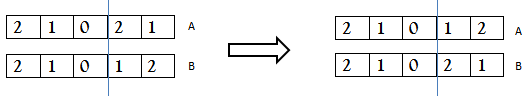
\includegraphics[scale=.5]{images/cross_over_fig.png}
				\caption{Illustration du croisement utilisé}
				\label{fig:used_cross_over}
			\end{center}
		\end{figure}
		
		\hspace*{.5cm} Le croisement se fait ainsi après la troisième période. Le croisement peut engendrer des individus qui, contrairement à la figure \ref{fig:used_cross_over}, ne respectent pas les contraintes de système en terme de \emph{shortage} ou de \emph{backlogging}. Il faut alors rendre ces individus à nouveau faisables avant de procéder à une quelconque mutation. L'algorithme \ref{alg:cross_over} présente le croisement implémenté dans le cadre de cette étude. Notons que notre algorithme a une complexité linéaire en $O(n)$\\
		
		\begin{algorithm}[H]
 		\caption{Algorithme de croisement utilisé}
 		\label{alg:cross_over}
 		\KwData{parent1, parent2, seuil\_probabilite}
 		\KwResult{child1 et child2}
 		\BlankLine
 		child1 $\gets$ $nouveau\ chromosome()$ \\
 		child2 $\gets$ $nouveau\ chromosome()$ \\
 		$probabilite \gets random(1,99)$ \\
 		\BlankLine
 		\If{probabilite $\leq$ seuil\_probabilite}
 		{
 			$nbGenes \gets NombreDeGenes(parent1)$\\
 			$indice\_gene \gets random(1, nbGenes)$\\
 			//$ Le \ nombre \ de \ genes \ du \ parent1 \ est \ le \ meme \ que \ celui \ du \ parent2 $\\
 			\For{ i $\gets$ 0 \KwTo nbGenes}
 			{
 				$gene1 \gets getGene(parent1, i)$ \\
 				$gene2 \gets getGene(parent2, i)$ \\
 				\eIf{i $\leq$ indice\_gene}
 				{
 					$child1.ajouterGene(gene)$ \\
 					$child2.ajouterGene(gene)$ \\
 				}
 				{
 					$child2.ajouterGene(gene)$ \\
 					$child1.ajouterGene(gene)$ \\
 				}
 			}
 		}
 		\Return{child1, child2}
		\end{algorithm}
		  
	\subsubsection{Mutation}
	Après la sélection et le croisement, une nouvelle population d'individus est prête. Certains ont été copiés directement et d'autres se sont reproduits par croisement. Dans le but de s'assurer que les individus ne sont pas exactement les mêmes, une mutation est appliquée à chacun des individus "\emph{fils}". A chaque gène, on attribue une chance de muter. Dans le cas, où la mutation se produit, la valeur du gène muté change de période. Un visuel de la mutation est présenté à la figure \ref{fig:used_mutation}. La mutation est un élément vital de la garantie d'une diversité au sein de la population. L'algorithme \ref{alg:mutation} détaille le processus utilisé afin de faire muter un chromosome. 
	
	\begin{figure}[!h]
		\begin{center}
			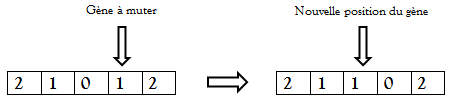
\includegraphics[scale=.5]{images/mutation_fig.png}
			\caption{Illustration de la méthode de mutation}
			\label{fig:used_mutation}
		\end{center}
	\end{figure}
	
	\begin{algorithm}[H]
 		\caption{Algorithme de mutation utilisé}
 		\label{alg:mutation}
 		\KwData{chromosome, seuil\_probabilite}
 		\KwResult{chromosome}
 		\BlankLine
 		$probabilite \gets random(1,99)$ \\
 		\BlankLine
 		\If{probabilite $\leq$ seuil\_probabilite}
 		{
 			\BlankLine
 			$nbGenes \gets NombreDeGenes(chromosome)$\\
 			\BlankLine
 			$indice\_gene \gets random(1, nbGenes)$\\
 			\BlankLine
 			$gene1 \gets getGene(chromosome, indice\_gene)$ \\
 			\BlankLine
 			//$ Le \ nombre \ de \ genes \ du \ parent1 \ est \ le \ meme \ que \ celui \ du \ parent2 $\\
 			\BlankLine
 			\For{ i $\gets$ indice\_gene \KwTo 0}
 			{
 				\BlankLine
 				$gene2 \gets getGene(chromosome, i)$\\
 				\BlankLine
 				\If{deadline(gene2) $>=$ indice\_gene}
 				{
 					\BlankLine
 					$deplacer(gene1, gene2, chromosome)$ \\
 					\BlankLine
 					$arret$
 					\BlankLine
 				}
 			}
 		}
 		\Return{chromosome}
		\end{algorithm}
	
	\subsection{Évaluation}
	L'évaluation dans notre étude, se réfère à la fonction objectif. Il s'agit de minimiser les coûts d'exploitation et de production. Deux types de coût sont à prendre en compte:
	\begin{itemize}
		\item[•] Les coûts de preparation ou \emph{setup} sont des coûts induits au moment d'un changement dans la configuration d'une ressource d'un type d'article à un autre. Il s'agit de perte potentielle de production durant la période de préparation, de force de travail additionnelle ou encore de ressources additionnelles brutes consommées durant la préparation.
		\item[•] Les coûts de stockage qui sont induits lors du conditionnement et d’entreposage.
	\end{itemize}
	L'algorithme \ref{alg:evaluation} explicite le processus suivi afin d'évaluer un chromosome.
	
	\begin{algorithm}[H]
 		\caption{Algorithme utilisé dans le processus d'évaluation d'un chromosome}
 		\label{alg:evaluation}
 		\KwData{chromosome, cout\_stockage, cout\_transition}
 		\KwResult{eval}
 		\BlankLine
 		$eval \gets 0$\\
 		$// On\ calcule\ le\ cout\ de\ stockage\ de\ chaque\ production$ \\
 		\For{gene in chromosome}{
 			\If{gene.value != 0}{		
 				$date\_limite \gets getDateLimite(gene)$ \\
 				$temp \gets (date\_limite\ -\ gene.periode) * cout\_stockage(gene.value)$ \\
 				$evaluation \gets evaluation\ +\ temp$ \\
 			}
 		}
 		$// On\ calcule\ le\ cout\ de\ transition\ de\ entre\ deux\ productions$ \\
 		\For{gene in chromosome}{
 			\If{gene.value != 0}{		
 				$next\_gene \gets getNextGene(chromosome)$ \\
 				\If{transition(gene, next\_gene) est vrai}{
 					$temp \gets cout\_transition(gene, next\_gene)$\\
 					$evaluation \gets evaluation\ +\ temp$
 				}
 			}
 		}
 		\Return{evaluation}
	\end{algorithm}
	
	\subsection{Terminaison}
	Deux moyens sont utilisés par lesquels les algorithmes génétiques se terminent. Habituellement, une limite est mise sur le nombre de générations après lesquelles le processus se termine. Avec certains problèmes, le processus de recherche se termine quand une solution particulière a été trouvée ou encore lorsque la plus haute valeur de "fitness" dans la population a atteint une valeur particulière. \\
	\hspace*{.5cm} Le critère de terminaison utilisé dans notre étude afin de terminer une recherche est le suivant : la recherche se termine lorsque l'algorithme converge sur un individu considéré comme une solution optimale. A cet optimal local, est appliqué une fonction de recherche locale afin de déterminer dans l'entourage immédiat de cet individu, un autre individu de meilleure qualité. Dans le cas, où un meilleur individu ne serait pas trouvé, la recherche s’arrête donc sur cet optimal local.
	
	\subsection{Fonction de faisabilité}
	Le croisement et la mutation sont tous des opérateurs génétiques qui produisent en sortie des chromosomes. En fonction du gène muté dans le cas de la mutation ou du point de croisement dans le cas du croisement, ces chromosomes peuvent ne pas être faisables; c'est-à-dire qu'ils ne représentent pas des solutions au problème à résoudre. Il importe donc de rendre à nouveau faisable. La fonction de faisabilité permet de rendre un chromosome ou individu à nouveau faisable. Afin d'y parvenir, nous avons réduit le surplus de production dans le cas d'un surplus et augmenter la quantité d'articles produits dans le cas d'un manque de production. L'algorithme \ref{alg:faisabilite} est celui utilisé dans cet objectif. 
	\\
	\begin{algorithm}[H]
 		\caption{Algorithme utilisé comme fonction de faisabilité}
 		\label{alg:faisabilite}
 		\KwData{chromosome, cout\_stockage, cout\_transition}
 		\KwResult{eval}
 		\BlankLine
 		$eval \gets 0$\\
 		$// On\ calcule\ le\ cout\ de\ stockage\ de\ chaque\ production$ \\
 		\For{gene in chromosome}{
 			\If{gene.value != 0}{		
 				$date\_limite \gets getDateLimite(gene)$ \\
 				$temp \gets (date\_limite\ -\ gene.periode) * cout\_stockage(gene.value)$ \\
 				$evaluation \gets evaluation\ +\ temp$ \\
 			}
 		}
 		$// On\ calcule\ le\ cout\ de\ transition\ de\ entre\ deux\ productions$ \\
 		\For{gene in chromosome}{
 			\If{gene.value != 0}{		
 				$next\_gene \gets getNextGene(chromosome)$ \\
 				\If{transition(gene, next\_gene) est vrai}{
 					$temp \gets cout\_transition(gene, next\_gene)$\\
 					$evaluation \gets evaluation\ +\ temp$
 				}
 			}
 		}
 		\Return{evaluation}
	\end{algorithm}
	
	\section{Méthodes de recherche proposées}	
	
	Les algorithmes génétiques sont des techniques de recherche qui ont été utilisées avec succès dans la résolution de problèmes dans différents disciplines. Cependant, la recherche permanente de performance dans l'exécution des algorithmes et le dévelop-pement constant d'ordinateurs toujours plus performants et parallèles ont conduit à l'émergence d'un type d'algorithmes génétiques plus performants que les algorithmes génétiques standards. A propos des algorithmes génétiques parallèles, on distingue généralement trois classes : les "\emph{master-slave} parallel genetic algorithms", les "\emph{ coarsed-grained} parallel genetic algorithms" et les "\emph{fine-grained} parallel genetic algorithms". Les "master-slave parallel genetic algorithms" sont le type le plus simple d'algorithmes génétiques parallèles. Elles consistent essentiellement à distribuer l'évaluation de la population globale entre plusieurs processeurs. Le processeur qui conserve la population et exécute l'algorithme génétique est le maître et les processus qui évaluent la population sont les esclaves. La figure \ref{fig:master_slave_ga} montre un schéma de l'algorithme génétique parallèle "master-slave". Nous nous intéressons dans notre étude aux deux autres types, plus compliqués mais également plus intéressants dans leur fonctionnement et performances.
	
	\begin{figure}[!h]
		\begin{center}
			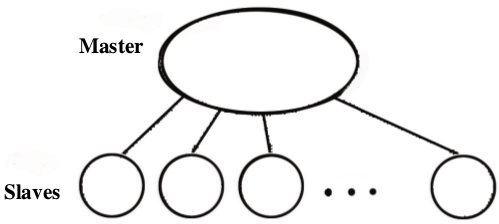
\includegraphics[scale=.3]{images/master_slave_ga.png}
			\caption{Schéma d'un algorithme génétique de type "master-slave" \cite{cant}}
			\label{fig:master_slave_ga}
		\end{center}
	\end{figure}
	
	\subsection{Algorithmes génétiques parallèles de type "\emph{coarse-grained}"}
	Les algorithmes génétiques de type "\emph{coarse-grained}" ou encore "\emph{modèle de l'île}" consiste en un ensemble de sous-populations qui échangent des individus de manière fréquente. Il s'agit probablement du type d'algorithmes génétiques le plus populaire bien qu'il nécessite de contrôler beaucoup de paramètres. La complète compréhension des effets de ces paramètres sur la qualité et la vitesse de recherche nous échappe encore. Cependant, Il a été démontré théoriquement que plus de sous-populations sont utilisées, leur taille peut être réduite sans sacrifier la qualité de la recherche. Vu que chaque processus s'exécute en parallèle, il en résulte une réduction du temps dédié aux calculs. Cependant, utiliser plus de sous-populations et donc de processus augmente la communication dans le système. Un compromis doit donc être effectué entre le temps de calculs et le temps de communication. L'implémentation des algorithmes génétiques parallèles soulève générale trois problématiques principalement sur la migration qui est l'échange d'individus entre processus. Il s'agit: de la fréquence de migration, du nombre d'individus à échanger, de la topologie des connections entre processus et de la méthode d'intégration des migrants.
	\subsubsection{Fréquence de migration}
	La migration affecte la qualité de la recherche et l'efficacité de l'algorithme en plusieurs points. Ainsi, de fréquentes migrations entraînent l'échange massif de potentiellement bons matériels génétiques, mais il affecte aussi négativement la performance dans le mesure où les communications sont coûteuses. La même chose se produit dans les topologies densément connectées où chaque processus communique avec les autres. Le but ultime des algorithmes génétiques parallèles est de trouver de bonnes solutions assez rapidement. Il est donc nécessaire de trouver l'équilibre entre le coût de la migration et l'augmentation des chances de trouver de bonnes solutions. \\
	\hspace*{.5cm} Afin d'implémenter l'algorithme, nous avons donné à l'utilisateur la possibilité d'entrer l'intervalle de générations en les migrations. Cependant, le comportement par défaut de l'algorithme est de migrer uniquement lorsque la population a convergé complètement.  
	\subsubsection{Nombre de migrants}
	La migration envoie un nombre prédéterminé d'individus d'un processus à ces processus voisins logiques sur le graphe de communications. Ces individus ou "\emph{migrants}" seront ainsi intégrés dans la population des processus auxquels ils ont été envoyés. Il est possible de choisir les "migrants" de façon aléatoire ou alors parmi les meilleurs individus de la population actuelle. La sélection aléatoire a l'avantage de disséminer plus de diversité et les chances d'explorer de nouvelles régions de l'espace de recherche peuvent être améliorées. La sélection des meilleurs individus peut aider à disséminer un matériel génétique qui a déjà été testé et qui serait donc intéressant. Dans la suite de notre étude, nous avons choisi d'échanger les meilleurs individus.
	\subsubsection{Topologie de connections}
	La topologie est également une importante partie des algorithmes génétiques de type \emph{"coarse-grained"}. En théorie, toute les topologies arbitraires peuvent être utilisées. Cependant, certains modèles sont fréquents. il s'agit : des topologies linéaires, des anneaux, des hypercubes. des densément connectés, des isolés. La topologie utilisée a été celle densément connectée présentée à la figure \ref{fig:topology_fig} 
	
	\begin{figure}[!h]
		\begin{center}
			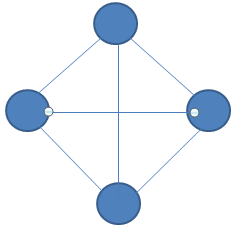
\includegraphics[scale=.3]{images/topology_fig.png}
			\caption{Topologie de connections utilisée}
			\label{fig:topology_fig}
		\end{center}
	\end{figure}
	
	\subsubsection{Méthode d'intégration des migrants}
 	Différentes alternatives existent pour incorporer les "\emph{migrants}". Deux d'entre elles sont récurrentes. Il s'agit: du remplacement aléatoire des individus de la population actuelle par les "\emph{migrants}" et du remplacement compétitif ou élitiste. Dans le remplacement aléatoire, les individus devant être remplacés sont désignés de manière aléatoire. Dans le remplacement compétitif, seules les individus avec les plus mauvais scores de "fitness" sont remplacés par les nouveaux arrivants. Un remplacement compétitif a été appliqué à notre programme. Il s'est agi d'identifier les plus mauvais chromosomes en terme de fitness et de les remplacer par les nouveaux arrivants.\\
 	\subsubsection{Algorithme hiérarchique entre \emph{coarse-grained} et \emph{master-slave}}
 	\hspace*{.5cm} Une fois, ces problématiques abordées, la question de l'implémentation rapide des algorithmes génétiques parallèles de type "\emph{coarse-grained}" revient. Une des réponses serait en effet de combiner ce type d'algorithmes génétiques parallèles avec un autre type, le "\emph{master-slave}" par exemple. On obtient alors un nouvelle classe d'algorithmes génétiques parallèles que sont les algorithmes génétiques parallèles hiérarchiques avec au niveau supérieur un algorithme génétique parallèle de type \emph{coarse-grained} et au niveau inférieur un algorithme génétique parallèle de type \emph{master-slave} comme le présente la figure \ref{fig:hierarchical_gene1_fig}. Il s'agit ainsi de cette combinaison que nous avons utilisée pour notre implémentation du programme et nos tests.
 	
	\begin{figure}[!h]
		\begin{center}
			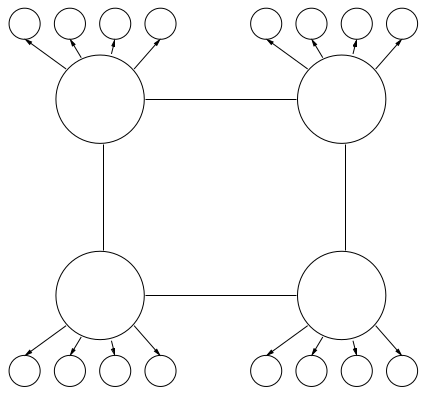
\includegraphics[scale=.3]{images/hierarchical_gene1_fig.png}
			\caption{Algorithmes génétiques parallèles et hierarchiques avec au niveau supérieur un algorithme génétique de type \emph{coarse-grained} et au niveau inférieur un algorithme génétique de type \emph{master-slave} \cite{cant2}}
			\label{fig:hierarchical_gene1_fig}
		\end{center}
	\end{figure} 	
 	
	\subsection{Algorithmes génétiques parallèles de type "\emph{fine-grained}"}
	les algorithmes génétiques parallèles de type "\emph{fine-grained}" ont seulement une population, mais la structure spatiale limite les interactions entre les individus. Un individu ne peut compétir et se reproduire qu'avec ses individus voisins. Vu que les voisinages se chevauchent, les bonnes solutions peuvent ainsi se disséminer à travers la population entière. Le choix le plus important dans l'implémentation de ce type d'algorithmes génétiques parallèles sont : la topologie de connections.
	\subsubsection{Topologie de connections}
	Différentes topologies de connections sont valables. Il s'agit entre autres des grilles 2-D, des hypercubes, le torus, le cube. Il est cependant répandu de placer les individus dans un algorithme génétique parallèle de type "\emph{fine-grained}" dans une grille 2-Dimension. En effet, dans la plupart des ordinateurs massivement parallèles, les éléments de traitement et de calculs sont connectés en suivant cette topologie. La figure \ref{fig:fine_grained_fig} présente la topologie utilisée afin d'implémenter l'algorithme génétique parallèle de type \emph{"fine-grained"}.
	
	\subsubsection{Principe de fonctionnement}
	Le principe de fonctionnement des algorithmes génétiques parallèles de type "\emph{fine-grained}" est différent de celui de type \emph{coarse-grained} et \emph{master-slave} est détaillé à l'algorithme \ref{alg:principe_fine_grained}. \\
	\\
	\begin{algorithm}[H]
 		\caption{Principe des algorithmes génétiques parallèles de type "\emph{fine-grained}" \cite{nayak}}
 		\label{alg:principe_fine_grained}
 		\BlankLine
 		\For{chaque nœud en parallèle}{
 		generer un individu de façon aléatoire
 		}
 		\BlankLine
 		\While{le critère de terminaison n'est pas satisfait}{
 			\For{chaque nœud en parallèle}{
 			evaluer le fitness de l'individu \\
 			obtenir la valeur de fitness des individus voisins \\
 			selectionner l'individu voisin dont la valeur de fitness est la plus grande \\
 			appliquer un croisement avec cet individu \\
 			muter l'individu qui en a résulté \\
 			}
 			Tester le critère de terminaison
 		}
	\end{algorithm}
	
	\begin{figure}[!h]
		\begin{center}
			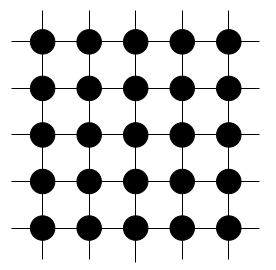
\includegraphics[scale=.3]{images/fine_grained_fig.png}
			\caption{Topologie utilisée en algorithme génétique parallèle de type "\emph{fine-grained}" \cite{cant2}}
			\label{fig:fine_grained_fig}
		\end{center}
	\end{figure} 
	
	\subsubsection{Algorithme hiérarchique entre \emph{fine-grained} et \emph{coarse-grained}}
	Des chercheurs ont combiné deux des méthodes de parallélisation produisant des algorithmes génétiques parallèles hiérarchiques. Certains de ces nouveaux algorithmes ajoutent un nouveau degré de complexité à des algorithmes déjà compliqués. On obtient alors des algorithmes génétiques parallèles hiérarchiques avec au niveau supérieur un algorithme génétique de type \emph{coarse-grained} et au niveau inférieur un algorithme génétique de type \emph{fine-grained} comme détaillé à la figure \ref{fig:hierar_fine_grained_fig}. Il s'agit en affet de notre deuxième proposition de méthode de résolution des instances de PSP que nous avons implémentée.
	
	\begin{figure}[!h]
		\begin{center}
			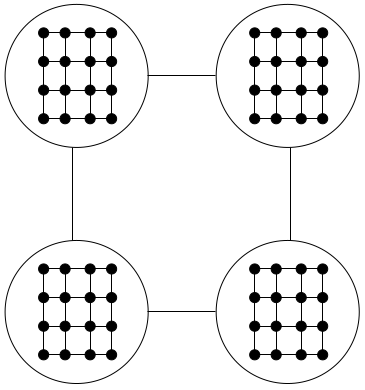
\includegraphics[scale=.3]{images/hierar_fine_grained_fig.png}
			\caption{Hiérarchie entre algorithmes génétiques parallèles de type \emph{fine-grained} et de type \emph{coarse-grained} \cite{cant2}}
			\label{fig:hierar_fine_grained_fig}
		\end{center}
	\end{figure} 
	
	\subsection{Autres algorithmes implémentés}
	Au cours de notre étude de l'art et en implémentant nos deux méthodes de résolution proposées que sont les algorithmes génétiques parallèles et hiérarchiques \emph{coarse-grained} et \emph{master-slave} et les algorithmes génétiques parallèles et hiérarchiques \emph{coarse-grained} et \emph{fine-grained}, nous avons pu découvrir différentes fonctions annexes aux algorithmes génétiques qui permettent d'en améliorer la qualité. Il s'agit des méthodes d'hybridation \cite{Goncalves} et de table de hashage \cite{povinelli}.
	
	\subsubsection{Hybridation}
	L'hybridation consiste à combiner deux méthodes de recherche afin d'engendrer une nouvelle méthode de recherche dit \emph{hybride}. Les algorithmes génétiques facilitent l'hybridation avec les autres techniques de recherche locale afin d'obtenir la solution optimale. De façon basique, la recherche locale et les algorithmes génétiques sont complémentaires. Les algorithmes génétiques sont efficaces lorsqu'il s'agit de parcourir un espace de recherche global, dans la mesure où elles sont capables de rapidement trouver des régions prometteuses. Cependant, elles prennent relativement beaucoup de temps à trouver des optimums dans ces régions. La recherche locale est capable de trouver des optimums avec une grande précision. \\
	\hspace*{.5cm} Dans notre étude, Nous avons mis au point un algorithme de recherche locale qui est utilisé à chaque fois que l'algorithme génétique converge sur une solution optimale afin de parcourir l'espace de recherche immédiat à cette solution et ainsi améliorer cette solution optimale. L'algorithme \ref{alg:local_search} décrit le processus suivi afin de chercher de meilleures solutions à partir d'un chromosome fourni en paramètre. Cet algorithme un complexité polynomiale en $O(n^{2})$ 
	\\
	\begin{algorithm}[H]
		\label{alg:local_search}
 		\caption{Algorithme de recherche locale d'une meilleure solution}
 		\KwData{individu à améliorer}
 		\BlankLine
 		\For{chaque gène du chromosome}{
 			\BlankLine
 			récupérer les coûts relatifs à la valeur de ce gène\\
 			\BlankLine
 			déterminer toutes les gènes à zéro respectant les contraintes liées à la valeur de ce gène.\\
 			\BlankLine
 			calculer le fitness du chromosome pour chaque gène à zéro\\
 			\BlankLine
 			choisir le gène à zéro qui maximise le fitness du chromosome \\
 			\BlankLine
 			insérer la valeur de l'item dans ce dernier gène\\ 
 			\BlankLine
 		}
	\end{algorithm}
	\vspace*{.5cm}
	Si on prend l'exemple du PSP en page \pageref{sec:problem_description} et qu'on applique cet algorithme au problème, on obtient la figure \ref{fig:local_search_fig}.
	
	\begin{figure}[!h]
		\begin{center}
			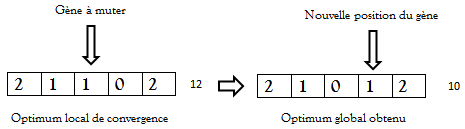
\includegraphics[scale=.6]{images/local_search_fig.png}
			\caption{Application de l'algorithme de recherche de meilleure solution à une chromosome}
			\label{fig:local_search_fig}
		\end{center}
	\end{figure} 
	
	\subsubsection{Table de Hash}
	Dans le processus de résolution des problèmes à l'aide algorithmes génétiques, au fur et à mesure que les générations passent, la population évolue et la diversité au sein de cette dernière diminue amenant les mêmes chromosomes à être régulièrement réévalués. Dans les faits, l'effort de calculs dépensé à évaluer le "\emph{fitness}" dépasse celui dépensé sur les opérateurs génétiques. En utilisant une table de hash afin de stocker les chromosomes récemment évalués, une amélioration significative des performances peut être constatée. Nous avons donc utilisé un dictionnaire ou tableau associatif afin de stocker ces derniers.
	
	\section*{Conclusion}
	\addcontentsline{toc}{section}{Conclusion}
	Cette deuxième partie a présenté le modèle utilisé dans la résolution du PSP ainsi que les aspects communs aux deux solutions proposées. Dans un second temps, nous avons présenté et détaillé deux approches heuristiques basées sur les algorithmes génétiques parallèles utilisées afin de résoudre le problème. Dans la suite, nous présentons nos deux approches et analysons les résultats afin de les comparer à l'état de l'art en la matière.
